\chapter{\difficult{Higher-dimensional Geometry}}\label{chapter:hdg}

    In this chapter we generalize certain constructions and theorems introduced in the previous chapters to the setting of higher categories. As such it can been as an analogue to chapter \ref{chapter:hda} for (differential) geometry.

    The main references are \cite{higher_gauge, phd_schreiber}. For a refresher on (higher) category theory see chapter \ref{chapter:cat}. Section \ref{section:higher_lie_structures} gives a different approach to the higher-dimensional analogues of Lie algebras.

    ?? CITE BAEZ, SCHREIBER, BARTELS, ... ??

\section{Smooth spaces}\label{section:smooth_spaces}
\subsection{Diffeological spaces}

    \newdef{Diffeological space}{\index{diffeology}\index{plot}
        Let $X$ be a set. A diffeology $\mathcal{D}$ on $X$ is defined as a collection of maps $f:U\subseteq\mathbb{R}^n\rightarrow X$, called \textbf{plots}, satisfying the following conditions (where $U,V$ and $W$ are open sets):
        \begin{enumerate}
            \item If $f$ is constant, then $f\in\mathcal{D}$.
            \item If $\{U_i\}_{i\in I}$ is an open cover of $U$ and if $f|_{U_i}\in\mathcal{D}$ for all $i\in I$, then $f\in\mathcal{D}$.
            \item If $f\in\mathcal{D}$ and $g:W\subseteq\mathbb{R}^m\rightarrow\dom(f)$ is smooth, then $f\circ g\in\mathcal{D}$.
        \end{enumerate}
        The set $X$ can be turned into a topological space by equipping it with the \textbf{$\mathcal{D}$-topology}, i.e. the final topology with respect to $\mathcal{D}$.
    }
    \remark{The domain of different plots can be subsets of different Euclidean spaces $\mathbb{R}^m$ and $\mathbb{R}^n$.}

    \newdef{Smooth map}{\index{smooth!function}
        \nomenclature[S_DiffSp]{$\mathbf{DiffSp}$}{category of diffeological spaces and smooth maps}
        Let $(X,\mathcal{D})$ and $(Y,\mathcal{D}')$ be diffeological spaces. A map $g:X\rightarrow Y$ is said to be smooth if for every $f\in\mathcal{D}$ the composition $g\circ f\in\mathcal{D}'$.

        The diffeological spaces together with their differentiable morphisms form a category $\mathbf{DiffSp}$.
    }

    \newdef{Chen space}{\index{Chen space}
        If we replace the open sets $U$ in the definition of a diffeological space by convex sets, we obtain a notion of smooth space due to Chen.
    }

    \begin{adefinition}[Manifold]\index{manifold}
        Let $M$ be a diffeological space. $M$ is called an $n$-manifold if it is locally diffeomorphic to $\mathbb{R}^n$.
    \end{adefinition}

    \begin{notation}[Smooth spaces]
        \nomenclature[S_Cinf]{$\mathbf{C^\infty}$}{category of smooth spaces}
        We will denote the category of smooth spaces (whatever model we might use) by $\mathbf{C^\infty}$.
    \end{notation}

\subsection{Smooth algebras}

    \newdef{Smooth algebra}{\index{smooth!algebra}
        \nomenclature[S_CSmAlg]{$\textbf{C}^\infty\textbf{Ring}$, $C^\infty$\textbf{Alg}}{category of smooth algebras}
        For any smooth manifold $M$ we have that \[C^\infty(M) \equiv C^\infty(M, \mathbb{R}) = \hom_{\mathbf{Diff}}(X, \mathbb{R}).\] Since hom-functors are (finite) product-preserving, we see that the multiplication $C^\infty(M)\times C^\infty(M)\rightarrow C^\infty(M)$ is induced by the multiplication on $\mathbb{R}$: $C^\infty(M, \mathbb{R}\times\mathbb{R})\cong C^\infty(M)\times C^\infty(M)$. At the same time the hom-functor is covariant in the second argument and hence we obtain a copresheaf on the category \textbf{CartSp}$_{\textbf{diff}}$ of Euclidean (Cartesian) spaces and smooth morphisms. Generalizing this situation we define smooth algebras as finite product-preserving copresheaves on \textbf{CartSp}$_{\textbf{diff}}$. This (functor) category is denoted by $\textbf{C}^\infty$\textbf{Alg}.
    }

    \newdef{Finitely generated smooth algebra}{\index{smooth!locus}
        Since ordinary $R$-algebras are finitely generated if and only if they are of the form $R[x_1,\ldots,x_k]/J$ for some integer $k\in\mathbb{N}$ and some ideal $J$, we define a finitely generated smooth algebra if it is of the form $C^\infty(\mathbb{R}^n)/J$ for some $n\in\mathbb{N}$ and some ideal $J$ in the ordinary ring underlying the smooth algebra.

        If we denote the category of finitely generated smooth algebras by $\textbf{C}^\infty\mathbf{Alg}^{\textbf{fin}}$, we can define the category of \textbf{smooth loci} as $(\textbf{C}^\infty\mathbf{Alg}^{\textbf{fin}})^{op}$. This generalizes the content of algebraic geometry (chapter \ref{chapter:alggeom}) to the ''smooth'' setting.
    }

\section{Higher geometry}

    In this section we extend the notions of groups, Lie groups and groupoids (introduced in sections \ref{section:groups}, \ref{section:lie_groups} and \ref{section:groupoids} respectively) the setting of higher category theory.

\subsection{Groups}

    \newdef{Lie groupoid\footnotemark}{\index{Lie!groupoid}\label{hdg:lie_groupoid}
        \footnotetext{Similarly one can define \textit{topological groupoids, \'etal\'e groupoids}, ...}
        A groupoid internal to $\mathbf{Diff}$. However, definition \ref{cat:internal_category} requires the existence of pullbacks (of the source and target morphisms). In the category $\mathbf{Diff}$ this is equivalent to assuming that the source and target morphisms are (surjective) submersions.
    }
    \remark{In the Ehresmannian approach one gives the manifold of composable morphisms $D_1\times_{D_0}D_1$ as part of the data. Hence we do not have to assume anything about the source and target morphisms.}

    \newdef{Lie algebroid}{\index{Lie!algebroid}\index{anchor}
        A vector bundle $\pi:E\rightarrow M$ together with a vector bundle morphism $\rho:E\rightarrow TM$, called the \textbf{anchor map}, and a Lie bracket on $\Gamma(E)$ such that the following Leibniz-type property is satisfied:
        \begin{gather}
            [X, fY] = f[X, Y] + \rho(X)(f)Y.
        \end{gather}
        This property also implies that $\rho$ preserves the Lie bracket:
        \begin{gather}
            \rho([X, Y]) = [\rho(X), \rho(Y)].
        \end{gather}
    }
    \begin{example}[Tangent Lie algebroid]\index{pair!groupoid}
        The tangent bundle over a smooth manifold is a Lie algebroid with $\rho\equiv\text{id}$.

        Both the fundamental groupoid $\mathbf{\Pi_1}(M)$ (see definition \ref{topology:fundamental_groupoid}) and the pair groupoid\footnote{The objects are the elements of $M$ and between every two objects there exists exactly one morphism, i.e. $\text{hom}(\mathbf{M\times M})\equiv M\times M$.} $\mathbf{M\times M}$ integrate the tangent Lie algebroid.
    \end{example}

    \newdef{Weak 2-group}{\index{group!categorical}\index{2!group}
        Let $(\mathbf{C},\otimes,\mathbf{1})$ be a monoidal category. This category is called a weak 2-group, \textbf{categorical group} or \textbf{gr-category} if it satisfies the following conditions:
        \begin{itemize}
            \item All morphisms are invertible.
            \item Every object is weakly invertible with respect to the monoidal structure.
        \end{itemize}
        By property \ref{cat:monoidal_or_2} one can equivalently define a weak 2-group as a 2-category with a single object, weakly invertible 1-morphisms and invertible 2-morphisms.
    }

    \newdef{2-groupoid}{\index{2!groupoid}
        A 2-groupoid is a 2-category in which all 1-morphisms are invertible and every 2-morphisms has a ''vertical'' inverse. (The ''horizontal'' inverse can be constructed from the other ones.)
    }
    \newdef{$\infty$-groupoid}{
        A $\infty$-category in which all morphisms are invertible. This is equivalent to a $(\infty,0)$-category in the language of $(n,r)$-categories.
    }

    \newdef{Strict 2-group}{
        A (strict) 2-group is defined as a (strict) 2-groupoid with only one object. From this it follows that the set of 1-morphisms forms a group and so does the set of 2-morphisms under horizontal composition. However, the 2-morphisms do not form a group under vertical composition\footnote{Because the sources/targets may not match up.}.

        This definition is equivalent to the following internal version: a (strict) 2-group is a group object in $\mathbf{Cat}$ or an internal category in $\mathbf{Grp}$. If we replace $\mathbf{Grp}$ by $\mathbf{Lie}$ we obtain the notion of a (strict) Lie 2-group.
    }

    \begin{property}[Lie crossed modules]\index{module!crossed}\index{differential!crossed module}
        The 2-category of (strict) 2-groups is biequivalent to the 2-category of (Lie) crossed modules \ref{group:crossed_module}. Given a 2-group $\mathcal{G}$ one obtains a crossed module as follows:
        \begin{itemize}
            \item $G:=\text{ob}(\mathcal{G})$,
            \item $H:=\{h\in\text{hom}(\mathcal{G}):\mathfrak{s}(f)=e\}$,
            \item $t(h):=\mathfrak{t}(h)$, and
            \item $\alpha(g)h := \mathbbm{1}_gh\mathbbm{1}_g^{-1}$
        \end{itemize}
        where $\mathfrak{s},\mathfrak{t}$ are the source and target morphisms in $\mathcal{G}$.

        To every Lie crossed module we can also assign a \textbf{differential crossed module}. This consists of the following data:
        \begin{enumerate}
            \item two Lie algebras $\mathfrak{g},\mathfrak{h}$,
            \item a Lie algebra morphism $\partial:\mathfrak{h}\rightarrow\mathfrak{g}$, and
            \item a Lie algebra morphism $\rho:\mathfrak{g}\rightarrow\text{Der}(\mathfrak{h})$.
        \end{enumerate}
        The equivariance and Peiffer conditions induce similar conditions for the above data:
        \begin{itemize}
            \item $\partial(\rho(h)g) = [h,\partial g]$, and
            \item $\rho(\partial h)(h') = [h,h']$
        \end{itemize}
        where $g\in\mathfrak{g}$ and $h,h'\in\mathfrak{h}$. The biequivalence of crossed modules and strict 2-groups induces a biequivalence of differential crossed modules and strict Lie 2-algebras.
    \end{property}

    \begin{example}[Automorphism 2-group]
        Given a Lie group $H$ one can construct a crossed module with $G:=\text{Aut}(H)$, $t$ assigning inner automorphisms (conjugations) and $\alpha$ the obvious map. The associated 2-group $\text{AUT}(H)$ gives a 2-group of symmetries of $H$, i.e. it is the automorphism 2-group of $H$ in the 2-category $\mathbf{Lie}$.
    \end{example}

    \newdef{Exponentiable groups}{\index{exponentiable}
        Smooth groups for which every smooth function $f:[0,1]\rightarrow\mathfrak{g}$ corresponds to a smooth function $g:[0,1]\rightarrow G$ such that
        \begin{gather}
            \deriv{}{t}g(t) = f(t)g(t)
        \end{gather}
        with $g(0) = e$, are said to be exponentiable. A smooth 2-group is said to be exponentiable if both of its component groups are exponentiable. Since all Lie groups are exponentiable, all Lie 2-groups are also exponentiable
    }

    \begin{remark}[Lie's third theorem]\index{Lie!third theorem}
        In ordinary Lie theory Lie's third theorem states that every (finite-dimensional) Lie algebra can be obtained as the infinitesimal version of a Lie group. However, this does not carry over to the 2-group setting. Consider for example the Lie 2-algebras $\mathfrak{g}_\lambda$ constructed in example \ref{hda:gk_lie_2_algebra}. As shown in \cite{HDA5} only $\mathfrak{g}_0$ gives rise to a Lie 2-group (or even a topological 2-group).
    \end{remark}

\subsection{Spaces}

    \newdef{Smooth 2-space}{
        To overcome the problem encountered in definition \ref{hdg:lie_groupoid} above, we should pass from $\mathbf{Diff}$ to $\mathbf{C^\infty}$. It can be shown that this category admits all pullbacks, quotients, path spaces, etc. As such we define a smooth 2-space as a category internal to $\mathbf{C^\infty}$.

        In the remainder of this chapter we will assume all spaces to be smooth in the general sense. The notions of 2-groups as introduced in the previous section are easily generalized to this wider setting.
    }

    \newdef{2-group action}{\index{group!action}
        Consider a smooth 2-group $\mathcal{G}$ and a smooth 2-space $E$. A strict action of $\mathcal{G}$ on $E$ is a smooth homomorphism $\mathcal{G}\rightarrow\text{AUT}(E)$, i.e. a smooth map preserving products and inverses.
    }

    \newdef{Thin homotopy}{\index{homotopy!thin}
        Let $M$ be a smooth manifold. A smooth homotopy $H:[0,1]^2\rightarrow M$ is said to be thin if
        \begin{gather}
            H(s, t) = F(s)
        \end{gather}
        for some smooth $F$ near $t=0,1$ and if it pulls back\footnote{See section \ref{diff:section:forms}.} every two-form to 0:
        \begin{gather}
            \forall \omega\in\Omega^2(M): H^*\omega = 0.
        \end{gather}
    }
    \newdef{Lazy path\footnotemark}{\index{path!lazy}\index{sitting instants}
        \footnotetext{Also called a path with \textbf{sitting instants}.}
        Let $M$ be a smooth manifold. A path $f:[0,1]\rightarrow M$ is said to be lazy if it is locally constant on some neighbourhoods of $0$ and $1$.
    }

    \newdef{Path groupoid}{\index{groupoid!path}\label{hdg:path_groupoid}
        Let $M$ be a smooth space. The path groupoid $\mathcal{P}_1(M)$ is the groupoid (in fact a smooth groupoid and hence a smooth 2-group) which has the points of $M$ as objects and the thin homotopy classes of lazy paths with fixed endpoints on $M$ as morphisms.\footnote{The laziness combined with the first condition of thin homotopies implies that the morphisms of the groupoid are (locally) constant near the full boundary of their domain.}

        In fact by suitably generalizing the smoothness properties of the homotopies and paths, we can ''easily'' extend this definition to surface, volumes and so on. This results in the $n$-path $n$-groupoid $\mathcal{P}_n(M)$.
    }
    \sremark{The restriction to lazy paths is required to ensure the smoothness of composite paths. The quotient by thin homotopies is required to ensure the validity of the associativity and invertibility properties.}

    ?? COMPLETE ??

\section{2-Bundles}

    A first step is the generalization of the categorical definition of a bundle \ref{diff:bundle}, i.e. as an object of a slice category:
    \newdef{2-bundle}{\index{bundle}
        A smooth 2-bundle is a triple $(E,B,\pi)$ where both $E$ and $B$ are smooth 2-spaces and $\pi$ is a smooth map.
    }
    \newdef{Locally trivial 2-bundle}{
        For a smooth 2-space we define a locally trivial 2-bundle with typical fibre $F$ as a 2-bundle $(E,B,\pi)$ with an open cover $\{U_i\}_{i\in I}$ of $B$ such that for every $i\in I$ there exists an equivalence $\varphi_i:E|_{U_i}\cong U_i\times F$ that makes the diagram below commute.

        \begin{figure}[ht!]
            \centering
            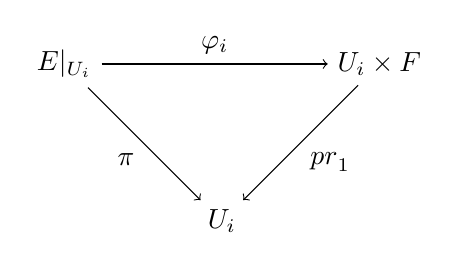
\begin{tikzpicture}
                \node (E) at (-2, 0) {$E|_{U_i}$};
                \node (UF) at (2, 0) {$U_i\times F$};
                \node (U) at (0, -2) {$U_i$};
                \draw[->] (E) -- node[above]{$\varphi_i$} (UF);
                \draw[->] (E) -- node[below left]{$\pi$} (U);
                \draw[->] (UF) -- node[below right]{$\text{pr}_1$} (U);
            \end{tikzpicture}
        \end{figure}
        We should note that the existence of such a cover is not a trivial matter. The general definition becomes quite involved when allowing for arbitrary smooth 2-spaces $B$. For convenience we will always assume that $B$ is an ordinary smooth space regarded as a 2-space with only trivial morphisms.

        As was the case in definition \ref{diff:fibre_bundle}, we can also characterize locally trivial 2-bundles by their transition data. Since the trivilizations $\varphi_i$ are equivalences, they admit an inverse (up to an invertible 2-map) and we can thus construct transition maps $\varphi_i\varphi_j^{-1}=U_{ij}\times F\cong U_{ij}\times F$ as usual. By the commutative diagram above, these transition maps only act on the fibre $F$. Because $\varphi_i\varphi_j^{-1}$ is itself an (auto)equivalence, the action on $F$ is given by a functor $g_{ij}:U_{ij}\rightarrow\text{AUT}(F)$ where the 2-space $\text{AUT}(F)$ is the \textit{coherent }2-\textit{group}\footnote{Instead of the strict invertibility of maps in our definition of 2-groups, we should allow them to be invertible up to 2-isomorphisms which themselves satisfy certain coherence conditions.} of autoequivalences of $F$ together with invertible 2-maps between them.

        The interesting (and important) part is how the cocycle conditions \ref{diff:G_cocycle_condition} and \ref{diff:G_cocycle_conditions} for the maps $g_{ij}$ are modified. Since the equivalences $g_{ij}$ are only invertible up to 2-maps, we cannot expect these conditions to hold as equations. Instead we obtain 2 higher transition maps (i.e. natural isomoprhisms) $h_{ijk}:g_{ij}\circ g_{jk}\Rightarrow g_{ik}$ and $k_i:g_{ii}\Rightarrow\text{id}$. These higher data should in turn satisfy the necessary conditions coming from associativity and unitality constraints (similar to the coherence conditions in section \ref{section:hda_group_cohomology}).
    }
    \newdef{$\mathcal{G}$-bundle}{\index{principal!bundle}
        A locally trivial 2-bundle with typical fibre $F$ is said to have the 2-group $\mathcal{G}$ as its structure (2-)group if the transition data factor through an action $\mathcal{G}\rightarrow\text{AUT}(F)$. If $F=\mathcal{G}$, we call the 2-bundle a \textbf{principal $\mathcal{G}$-2-bundle}.
    }
    \begin{remark}[Gerbes]\index{gerbe}
        If we choose the transition maps $k_i$ to be trivial and let $\mathcal{G}$ be respectively the trivial Lie 2-group associated to an Abelian Lie group $G$ or the automorphism 2-group of a Lie group $H$, we obtain Abelian and non-Abelian \textit{gerbes}. In fact it can be shown that the 2-category of principal $2$-bundles is equivalent to the 2-category of gerbes for every Lie 2-group of the aforementioned type.
    \end{remark}

    By categorifying definition \ref{diff:holonomy_functor} of principal connections we can define connections for principal $n$-bundles:
    \newdef{$n$-connection}{\index{connection!principal}
        Let $M$ be a smooth space and let $G$ be a Lie $n$-groupoid. Given a locally trivial principal $n$-bundle $P$ over $M$ we define an $n$-connection with $n$-holonomy through the following data:
        \begin{enumerate}
            \item for every coordinate chart $U_i\subset M$ a local holonomy $n$-functor
            \begin{gather}
                \text{hol}_i:\mathcal{P}_n(U_i)\rightarrow G;
            \end{gather}
            \item for every double intersection $U_{ij}$ a 1-transfor (i.e. an $n$-natural transformation)
            \begin{gather}
                g_{ij}:\text{hol}_i\Rightarrow\text{hol}_j;
            \end{gather}
            \item for every triple intersection $U_{ijk}$ a 2-transfor
            \begin{gather}
                f_{ijk}:g_{ij}\circ g_{jk}\Rrightarrow g_{ik};
            \end{gather}
            \item and so on...
        \end{enumerate}
        This is equivalently given by a global $n$-functor
        \begin{gather}
            \text{hol}:\mathcal{P}_n(M)\rightarrow\mathbf{Trans}_n(P).
        \end{gather}
    }

    ?? ADD GERBES (e.g. BRYLINSKI) AND PERHAPS DELIGNE COHOMOLOGY ??